


\tikzset{every picture/.style={line width=0.75pt}} %set default line width to 0.75pt        

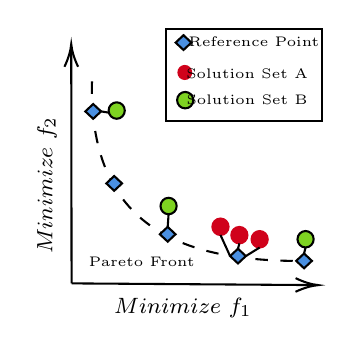
\begin{tikzpicture}[x=0.75pt,y=0.75pt,yscale=-1,xscale=1]
%uncomment if require: \path (0,235); %set diagram left start at 0, and has height of 235

%Straight Lines [id:da8717354133525324] 
\draw    (420.65,153.75) -- (420.49,40.47) ;
\draw [shift={(420.49,38.47)}, rotate = 449.92] [color={rgb, 255:red, 0; green, 0; blue, 0 }  ][line width=0.75]    (10.93,-3.29) .. controls (6.95,-1.4) and (3.31,-0.3) .. (0,0) .. controls (3.31,0.3) and (6.95,1.4) .. (10.93,3.29)   ;

%Straight Lines [id:da6788473220220854] 
\draw    (420.65,153.75) -- (537.5,154.57) ;
\draw [shift={(539.5,154.59)}, rotate = 180.4] [color={rgb, 255:red, 0; green, 0; blue, 0 }  ][line width=0.75]    (10.93,-3.29) .. controls (6.95,-1.4) and (3.31,-0.3) .. (0,0) .. controls (3.31,0.3) and (6.95,1.4) .. (10.93,3.29)   ;

%Curve Lines [id:da2578618754086526] 
\draw  [dash pattern={on 4.5pt off 4.5pt}]  (430.49,56.41) .. controls (428.85,130.62) and (479.36,143.75) .. (535.91,142.91) ;


%Shape: Ellipse [id:dp791999357308242] 
\draw  [color={rgb, 255:red, 208; green, 2; blue, 27 }  ,draw opacity=1 ][fill={rgb, 255:red, 208; green, 2; blue, 27 }  ,fill opacity=1 ] (488.5,126.47) .. controls (488.5,124.29) and (490.24,122.51) .. (492.39,122.51) .. controls (494.54,122.51) and (496.29,124.29) .. (496.29,126.47) .. controls (496.29,128.66) and (494.54,130.44) .. (492.39,130.44) .. controls (490.24,130.44) and (488.5,128.66) .. (488.5,126.47) -- cycle ;
%Shape: Ellipse [id:dp9676691887328452] 
\draw  [color={rgb, 255:red, 208; green, 2; blue, 27 }  ,draw opacity=1 ][fill={rgb, 255:red, 208; green, 2; blue, 27 }  ,fill opacity=1 ] (497.61,130.51) .. controls (497.61,128.33) and (499.35,126.55) .. (501.5,126.55) .. controls (503.65,126.55) and (505.39,128.33) .. (505.39,130.51) .. controls (505.39,132.7) and (503.65,134.47) .. (501.5,134.47) .. controls (499.35,134.47) and (497.61,132.7) .. (497.61,130.51) -- cycle ;
%Shape: Ellipse [id:dp5116089282119083] 
\draw  [color={rgb, 255:red, 208; green, 2; blue, 27 }  ,draw opacity=1 ][fill={rgb, 255:red, 208; green, 2; blue, 27 }  ,fill opacity=1 ] (507.37,132.51) .. controls (507.37,130.32) and (509.11,128.54) .. (511.27,128.54) .. controls (513.42,128.54) and (515.16,130.32) .. (515.16,132.51) .. controls (515.16,134.69) and (513.42,136.47) .. (511.27,136.47) .. controls (509.11,136.47) and (507.37,134.69) .. (507.37,132.51) -- cycle ;
%Shape: Diamond [id:dp9404744531551759] 
\draw  [color={rgb, 255:red, 0; green, 0; blue, 0 }  ,draw opacity=1 ][fill={rgb, 255:red, 74; green, 144; blue, 226 }  ,fill opacity=1 ] (431.07,67.34) -- (434.86,70.89) -- (431.07,74.45) -- (427.28,70.89) -- cycle ;
%Shape: Diamond [id:dp1840229468184298] 
\draw  [color={rgb, 255:red, 0; green, 0; blue, 0 }  ,draw opacity=1 ][fill={rgb, 255:red, 74; green, 144; blue, 226 }  ,fill opacity=1 ] (441.19,102.02) -- (444.98,105.58) -- (441.19,109.13) -- (437.4,105.58) -- cycle ;
%Shape: Diamond [id:dp7181430347383788] 
\draw  [color={rgb, 255:red, 0; green, 0; blue, 0 }  ,draw opacity=1 ][fill={rgb, 255:red, 74; green, 144; blue, 226 }  ,fill opacity=1 ] (466.96,126.53) -- (470.75,130.09) -- (466.96,133.64) -- (463.17,130.09) -- cycle ;
%Shape: Diamond [id:dp0076213596461021105] 
\draw  [color={rgb, 255:red, 0; green, 0; blue, 0 }  ,draw opacity=1 ][fill={rgb, 255:red, 74; green, 144; blue, 226 }  ,fill opacity=1 ] (500.83,137.04) -- (504.62,140.59) -- (500.83,144.15) -- (497.03,140.59) -- cycle ;
%Shape: Diamond [id:dp3966825993991798] 
\draw  [color={rgb, 255:red, 0; green, 0; blue, 0 }  ,draw opacity=1 ][fill={rgb, 255:red, 74; green, 144; blue, 226 }  ,fill opacity=1 ] (532.66,139.36) -- (536.46,142.91) -- (532.66,146.47) -- (528.87,142.91) -- cycle ;
%Shape: Ellipse [id:dp8366972743499659] 
\draw  [color={rgb, 255:red, 208; green, 2; blue, 27 }  ,draw opacity=1 ][fill={rgb, 255:red, 208; green, 2; blue, 27 }  ,fill opacity=1 ] (472.13,52.14) .. controls (472.13,50.41) and (473.5,49.01) .. (475.2,49.01) .. controls (476.9,49.01) and (478.27,50.41) .. (478.27,52.14) .. controls (478.27,53.86) and (476.9,55.26) .. (475.2,55.26) .. controls (473.5,55.26) and (472.13,53.86) .. (472.13,52.14) -- cycle ;
%Shape: Rectangle [id:dp9875854969558264] 
\draw   (465.98,31.31) -- (541.5,31.31) -- (541.5,75.72) -- (465.98,75.72) -- cycle ;
%Shape: Diamond [id:dp12687480943241192] 
\draw  [color={rgb, 255:red, 0; green, 0; blue, 0 }  ,draw opacity=1 ][fill={rgb, 255:red, 74; green, 144; blue, 226 }  ,fill opacity=1 ] (474.58,34.18) -- (478.38,37.74) -- (474.58,41.29) -- (470.79,37.74) -- cycle ;
%Shape: Ellipse [id:dp7460760771460382] 
\draw  [color={rgb, 255:red, 0; green, 0; blue, 0 }  ,draw opacity=1 ][fill={rgb, 255:red, 126; green, 211; blue, 33 }  ,fill opacity=1 ] (529.5,132.47) .. controls (529.5,130.29) and (531.24,128.51) .. (533.39,128.51) .. controls (535.54,128.51) and (537.29,130.29) .. (537.29,132.47) .. controls (537.29,134.66) and (535.54,136.44) .. (533.39,136.44) .. controls (531.24,136.44) and (529.5,134.66) .. (529.5,132.47) -- cycle ;
%Shape: Ellipse [id:dp8222601223763368] 
\draw  [color={rgb, 255:red, 0; green, 0; blue, 0 }  ,draw opacity=1 ][fill={rgb, 255:red, 126; green, 211; blue, 33 }  ,fill opacity=1 ] (438.5,70.47) .. controls (438.5,68.29) and (440.24,66.51) .. (442.39,66.51) .. controls (444.54,66.51) and (446.29,68.29) .. (446.29,70.47) .. controls (446.29,72.66) and (444.54,74.44) .. (442.39,74.44) .. controls (440.24,74.44) and (438.5,72.66) .. (438.5,70.47) -- cycle ;
%Shape: Ellipse [id:dp5535523746552888] 
\draw  [color={rgb, 255:red, 0; green, 0; blue, 0 }  ,draw opacity=1 ][fill={rgb, 255:red, 126; green, 211; blue, 33 }  ,fill opacity=1 ] (463.5,116.47) .. controls (463.5,114.29) and (465.24,112.51) .. (467.39,112.51) .. controls (469.54,112.51) and (471.29,114.29) .. (471.29,116.47) .. controls (471.29,118.66) and (469.54,120.44) .. (467.39,120.44) .. controls (465.24,120.44) and (463.5,118.66) .. (463.5,116.47) -- cycle ;
%Straight Lines [id:da3248368940477697] 
\draw    (434.86,70.89) -- (438.5,71.47) ;


%Straight Lines [id:da5912697186863101] 
\draw    (467.39,120.44) -- (466.96,126.53) ;


%Straight Lines [id:da6656789090734234] 
\draw    (533.39,136.44) -- (532.66,139.36) ;


%Straight Lines [id:da4766593569740376] 
\draw    (492.39,130.44) -- (497.03,140.59) ;


%Straight Lines [id:da5765204277329508] 
\draw    (501.5,134.47) -- (500.83,137.04) ;


%Straight Lines [id:da5373571677163032] 
\draw    (511.27,136.47) -- (504.62,140.59) ;


%Shape: Ellipse [id:dp9862032948376587] 
\draw  [color={rgb, 255:red, 0; green, 0; blue, 0 }  ,draw opacity=1 ][fill={rgb, 255:red, 126; green, 211; blue, 33 }  ,fill opacity=1 ] (471.5,65.47) .. controls (471.5,63.29) and (473.24,61.51) .. (475.39,61.51) .. controls (477.54,61.51) and (479.29,63.29) .. (479.29,65.47) .. controls (479.29,67.66) and (477.54,69.44) .. (475.39,69.44) .. controls (473.24,69.44) and (471.5,67.66) .. (471.5,65.47) -- cycle ;

% Text Node
\draw (474.34,165.66) node  [font=\footnotesize]  {$Minimize\ f_{1}$};
% Text Node
\draw (408.77,106.46) node  [font=\footnotesize,rotate=-270.12]  {$Minimize\ f_{2}$};
% Text Node
\draw (454.49,143.48) node  [font=\tiny] [align=left] {Pareto Front};
% Text Node
\draw (505.22,52.49) node  [font=\small] [align=left] {{\tiny Solution Set A}};
% Text Node
\draw (508.5,37.31) node  [font=\small] [align=left] {{\tiny Reference Point}};
% Text Node
\draw (505.22,65.49) node  [font=\small] [align=left] {{\tiny Solution Set B}};


\end{tikzpicture}
